%! TeX program = lualatex

\documentclass{juliacon}

\usepackage[labelfont=bf]{caption}
\captionsetup[table]{skip=4pt}
\captionsetup{font=scriptsize}

\usepackage{fontspec}
\usepackage{minted}

\newfontfamily \JuliaMono {JuliaMono.ttf}[
    Path      = ./,
    Extension = .ttf
    ]

\newfontface \JuliaMono{JuliaMono}

\setmonofont{JuliaMono}[
    Contextuals=Alternate
]

\setcounter{page}{1}

\begin{document}

% **************GENERATED FILE, DO NOT EDIT**************

\title{My JuliaCon proceeding}

\author[1]{Jacob S. Zelko}
\author[1, 2]{Malina Hy}
\author[1, 2]{Varshini Chinta}
\affil[1]{Georgia Tech Research Institute}
\affil[2]{Georgia Institute of Technology}

\keywords{Observational Health, OMOP Common Data Model, Database Management, Characterization}

\hypersetup{
pdftitle = {My JuliaCon proceeding},
pdfsubject = {JuliaCon 2019 Proceedings},
pdfauthor = {Jacob S. Zelko, Malina Hy, Varshini Chinta},
pdfkeywords = {Observational Health, OMOP Common Data Model, Database Management, Characterization},
}



\maketitle

\begin{abstract}

% TODO::HARD Review the abstract after reviewing the paper fully
Observational health continues to be a growing field in health informatics research as electronic health records (EHR), patient medical claims, and other ancilliary patient data source become more readily computable and accessible to researchers.
JuliaHealth is poised as an ecosystem to innovate within this area of research by bringing highly performant analytics approaches, composable solutions, and interoperable software that leverages prior state of the art. 
This paper will discuss the state of the art observational health research tools within the JuliaHealth ecosystem and how JuliaHealth is prepared to further research goals within this domain.

\end{abstract}

\section{Introduction}

% EXPLAIN::EASY What is observational health research?
% EXPLAIN::MEDIUM What sort of innovations?
Over the past $10$ years, there have been several innovations within the observational health research community.  Observational health research is an area of study that leverages authentic health data to gain insights into the health system without interference. Data are collected by researchers as they follow groups of people over a specified period. Depending on the study, these groups may comprise healthy individuals, individuals with a specific disease, or those at high risk of developing a particular condition—such as individuals with a family history—while also taking into consideration the imperative of safeguarding their privacy. Observational studies can contribute to answering questions as what genes cause a specific disease to grow, patterns and trends for a particular disease, experiences of past patients, behaviours increasing the risk of developing a certain disease. 

% EXPLAIN::MEDIUM Why is this a crucial innovation?
% EXPLAIN::MEDIUM What is meant by a transferable analysis?
Arguably, the most crucial innovation that has emerged is the Observational Medical Outcomes Partnership Common Data Model (OMOP CDM) which was designed specifically to standardize observational health data to enable transferable analyses. \cite{overhage2012validation}
% EXPLAIN::MEDIUM Why is mapping relevant here?
The importance of this model has become apparent within open science organizations like the OHDSI (Observational Health Data Science and Informatics) network where members across $100+$ countries \cite{sachsonOurJourney2023} with access to various health systems have been able to successfully map their patient data to the OMOP CDM.
% TODO::EASY Add citation about successful collaborations
% EXPLAIN::EASY What is a network study?
% TODO::EASY Cite the quote "write once, run everywhere" 
% http://www.sun.com/smi/Press/sunflash/1996-01/sunflash.960123.10561.xml} 
This has led to successful collaboration relationships across countries where one research group can develop a network study and then disseminate the study across collaborators leading to the idea that you can "write once, run everywhere."

\subsection{Core Technologies}

Modern observational health research centers around a variety of core technologies.
A few of these technologies highlighted in this paper are:

\begin{enumerate}

\item Data standards within observational health research
\item Collaborative networks and studies using observational health data
\item Research software to support the analysis of observational health data

\end{enumerate}

In particular, the data standard that will be most highlighted for the remainder of this paper is the Observational Medical Outcomes Partnership Common Data Model (OMOP CDM).
Subsequent discussion will be focused on the opportunities that this specific data model has given rise to across observational health as well as research communities such as the Observational Health Data Sciences and Informatics (OHDSI) open science consortium.

% TODO::MEDIUM This paragraph should be centered on the core technology of data standards -- in particular, the OMOP CDM
% EXPLAIN::MEDIUM What is real world data? Use https://jacobzelko.com/10282021140730-real-world-evidence/
OMOP was created in 2009 by the US Food and Drug Administration to address concerns related to data type, study design, and data privacy concerns of "Real World Data" \cite{ohdsi2019book} \cite{FDARealWorldEvidence}
What could arguably be considered the longest standing achievement of OMOP was the development of the OMOP Common Data Model (OMOP CDM) to house and ingest real world data.
% TODO::EASY Combine the next two sentences together
% EXPLAIN::EASY What does "person-centered" mean?
% EXPLAIN::MEDIUM What is a patient event? Could you give an example?
in a consistent format that has been optimized to assist in extracting meaningful population health information.
In brief, the OMOP Common Data Model (CDM) is a "person-centered" model that has standardized common events in a given patient encounter with database tables that represent the unique structures found in patient events.
% TODO::EASY Develop this fragment into a full sentence
prioritizing data protection through the limiting of information that could endanger patient anonymity.
% EXPLAIN:: What is a health system? Could you give an example?
This creates a longitudinal view of all healthcare-related events per person recorded in a singular health system.
% TODO::EASY Make this more coherent to the rest of the paragraph
% TODO::EASY Explicitly mention that although the model prescribes a database schema, it does not need a specific database type
The OMOP CDM itself does not require a specific technology to work with the data stored in this standard.

% TODO::MEDIUM This paragraph should be centered on the core technology of the concept of network studies
% TODO::MEDIUM Use this to address the notion of what "network studies" are
% TODO::MEDIUM Make this initially less OHDSI specific; pull from https://jacobzelko.com/05122023034151-network-macarthur
In particular, one collaboration mechanism that OHDSI has been able to operationalize meaningfully while working with observational health data is the notion of "network studies".
These studies, are designed to be transparent and encompasses research endeavors being explored by members of OHDSI comprehensive of relevant documentation, analysis code, results, and study protocols describing the study's scope and objectives.
OHDSI had its inception in the development of the Observational Medical Outcomes Partnership (OMOP) that was created in 2009 by the US Food and Drug Administration to address concerns related to data type, study design, and data privacy concerns of "Real World Data" \cite{ohdsi2019book} \cite{FDARealWorldEvidence}
OHDSI was developed to focus on leveraging observational health data stored within the OMOP CDM.
Since current observational health data sources are aggregated at different levels and cannot be generalized to the overall population, the data is often incomplete, inaccurate, and prone to issues of bias, error handling, and multidimensional complexity. 
The goal of OHDSI is to produce reproducible, robust, and reliable evidence by developing standardized data formats and research protocol designs to enable large-scale collaborative research and improve the transparency and scalability of observational health research. 
% TODO::MEDIUM Carry HADES discussion into the paragraph talking about research tooling
One core innovation brought about by OHDSI in the space of network science is how, given the HADES tools and procedures established by OHDSI, 
% TODO::EASY Make this more general such that it flows into the next paragraph on research tooling better
a research group can develop their analysis on their own OMOP CDM instance and then bundle together their study.
% EXPLAIN::EASY What is a study package?
% EXPLAIN::EASY What data assets?
Once this packaging is done, they can pass along the study package to another site to collaborate on the same analysis but on different data assets.
% EXPLAIN::MEDIUM What is a collaborator network?
Data confidentiality is preserved in this approach as data from individual participating sites remains exclusive to each site, with only aggregate results shared across a given collaborator network.
As such, no risk for re-identification comes about through this network collaboration and has ushered in the possibility for similar research approaches to be taken across the globe. \cite{ohdsi2019book}

% TODO::HARD Develop this paragraph more about research software
As the OMOP CDM has become ubiquitous within observational health research, developing research software to handle and manage OMOP CDM data is necessary to meaningfully contribute within the observational health research space.
OHDSI supports the development of open-source software tools in a centralized ecosystem called HADES (Health Analytics Data-to-Evidence Suite) for particularly managing and working with OMOP CDM formatted data.
The HADES ecosystem has been in existence for $\approx 10$ years and has given rise to improvements in the quality and reliability of observational health research as well as motivating novel collaboration mechanisms.

\subsection{JuliaHealth and Observational Health Research}

As JuliaHealth is an ad hoc network of contributors, varying aspects of the ecosystem have developed at differing rates as a function of factors such as developer time or workplace incentives.

At this time, OHS prioritizes creation and maintenance of tools that support analysis of "OMOP-ified"\footnotemark data (that is, data which is formatted in the OMOP CDM), in much the same manner that OHDSI does.

\footnotetext{It is unclear where terms like "OMOP-ify" or "OMOP-ification" (the process of converting a data to the OMOP CDM) originated; it may have been coined by Dr. Jon Duke.}

JuliaHealth is an open-science collective dedicated to bringing the Julia programming language to various avenues of health research domains including, but not limited to, observational health, medical imaging, standards interoperability and more.\cite{aluthgeAnnouncingJuliaHealthOrganization2020}
It leverages the strengths of the Julia language to introduce new methods into these spaces, augment existing workflows, and provide a community structure for health researchers within the global Julia ecosystem.
% EXPLAIN::EASY What is a subecosystem?
% EXPLAIN:: How does having more subecosystems enable novel research to be done?
Eventually, JuliaHealth will host a variety of subecosystems and associated resources that will enable novel research to be conducted within Julia. 

One area of the subecosystems within JuliaHealth that has matured significantly over the years has been the JuliaHealth observational health subecosystem (OHS).
It can be said that OHS had its inception in work done by Evans and Simonov with efforts such as \textit{FunOHDSI.jl} \cite{evansFunOHDSIJl2022}, \textit{OHDSICohortExpressions.jl} \cite{evansOHDSICohortExpressionsJl2023}, and \textit{FunSQL.jl} around $2021$ \cite{kirill_simonov_2023_7705325}
% TODO::EASY Cite OHDSI Symposium poster on JuliaHealth
% TODO::HARD Register OHDSI Symposium poster to Zenodo
% TODO::EASY Cite JuliaCon 2023 presentation
% TODO::HARD Register JuliaCon 2023 presentation to Zenodo
Since then, Zelko et. al. have spearheaded most recent developments within OHS via the creation of a variety of tools and demonstrated their effectiveness in using these tools for novel observational health research endeavors \cite{zelko2022pilot}
% EXPLAIN::MEDIUM What does this mean?
Through such efforts, OHS is becoming further capable of executing novel observational health research. 

\section{Accomplishing Common Observational Health Research Tasks within Julia}

JuliaHealth has capacity through the OHS to perform observational health workflows via a variety of tools designed to support and enable novel investigations.
This paper summarizes and highlights some of the current capacity OHS provides such as:

\begin{enumerate}
\item \textbf{Using Phenotype Definitions} - brief overview of phenotype definitions and how to work with them
\item \textbf{Rapid Cohort Iteration and Creation} - how to iteratively develop patient cohorts to explore
\item \textbf{Working with Patient Databases} - approaches to working with different patient databases
\item \textbf{Ecosystem Interoperability} - extending JuliaHealth's ecosystem to other research ecosystems
\end{enumerate}

\subsection{Using Phenotype Definitions}

% TODO::MEDIUM Add a paragraph here about what is a phenotype definition
% TODO::EASY Cite my paper here

% TODO::EASY Segue this better from phenotype definitions
One of the premier tools within the OHDSI HADES ecosystem is the ATLAS Shiny application which was developed to develop patient phenotype definitions within observational health research contexts (amongst other use cases).
These phenotype definitions have varying levels of complexity where they can be very simple (such as finding all patients with one health condition or diagnosis) or grow to be extremely complex (defining controlled, uncontrolled, and indeterminate patient cohorts based on medications, lab results, etc.)
% TODO::EASY Create footnote about schema
% TODO::EASY Add reference to schema in footnote
% TODO::EASY Cite reference schema from GitHub in footnote; \cite{madrilATLASJSONSchema2022}
% EXPLAIN::EASY Better introduce what SQL is
The computable phenotype definitions that ATLAS generates based on phenotype definitions are in a variety of serialization formats such as JSON or prepared SQL expressions available in multiple SQL flavors.

% TODO::MEDIUM Reframe this to more say how ATLAS can be used to build cohorts
% TODO::EASY Explain how this package accomplishes similar tasks
The Julia package, OHDSICohortExpressions.jl, exists specifically to ingest these serialized expressions of computable phenotype definitions and create patient cohorts that match the given criterion in the definition. \cite{evansOHDSICohortExpressionsJl2023}
% TODO::MEDIUM Turn all items into complete thoughts in list
How this tool works is to:

\begin{enumerate}

\item read and verify the serialized computable phenotype definition 

\item reinterpret the serialization into the FunSQL.jl Domain Specific Language 

\item return a prepared SQL statement against a given SQL database that queries an OMOP CDM database for the desired patient population(s) of interest.

\end{enumerate}

% EXPLAIN::MEDIUM What is a prepared statement?
% EXPLAIN::MEDIUM What is a cohort in this context?
Once these prepared statements are made, researchers can execute the generated SQL against their OMOP CDM instance to generate cohorts for future analyses.

\subsection{Rapid Cohort Iteration and Creation}

% TODO::EASY Reword this sentence
Although OHDSICohortExpressions.jl is sufficient to translate existing phenotype definitions generated in ATLAS to executable queries, oftentimes, there is a tricky problem of how to best iterate on phenotype definitions. \cite{zelkoDevelopingRobustComputable2023}
% EXPLAIN:: Better contextualize why this is important -- why not just create a new phenotype definition?
Often, one has to take an existing definition and either revise to a more narrow cohort or write manual code to build more niche cohorts after an initial definition is created.
% EXPLAIN::MEDIUM How so?
% TODO::MEDIUM Review this sentence; maybe cut it
This refactoring of a phenotype definition can lead to conflating ideas within conversation between expert clinical reviewers, analysts, and health researchers.
% TODO::EASY Move this to the previous section on phenotype definitions
This broadly can be the notions of what we are exploring (the phenotype definition; often the responsibility of a clinical reviewer), what is possible to compute upon (the computable phenotype definition; often the responsibility of an analyst), and the goals of the overall study.

% TODO::EASY Present this more as a general introduction to what tools are here for this
% TODO::EASY Talk about composition with DataFrames or Tidier
OMOPCDMCohortCreator.jl allows one to iteratively build a patient population quickly and easily.
One can use patient pools developed from pre-existing cohorts defined off of phenotype definitions as a starting point in exploring patients or create new patient populations quickly without the need for a well-defined phenotype definition.
% TODO::MEDIUM Mention the ability to satisfy research requests
This can enable analysts to more quickly understand what is inside their data assets, do "quick" analysis of a particular smaller research question, and enable a more distinct separation of work between a clinical expert reviewer and analyst teams.

\subsection{Working with Patient Databases}

One of the biggest styming factors within not only the Julia ecosystem, but observational health research in general has been the difficulty of working with different databases.\cite{zelko2023julia}
Although the OMOP CDM has been great for standardizing \textit{how} real world data is handled, there is a lack of consensus on \textit{what} is needed to handle these data assets.
% TODO::EASY Make this less verbose
For a variety of reasons, different groups will choose different database architectures (perhaps PostgreSQL for improved permission support, DuckDB for performance, or even SQLite for ease of use) but all are subtly different enough to create headaches in seamlessly working across different research sites.

% TODO::EASY Change the phrasing of this
The way that the Julia ecosystem handles this is via the creation of a common database interface called the DBInterface.
% EXPLAIN:: What is dispatch
Specific Julia database packages can implement dispatches for this interace allowing users to have a much better experience working across databases.
In spite of such benefits, for some users (and especially within the context of observational health studies), it can beneficial to have a more prescriptive interface where one just needs to pass perhaps a password, username, database name, and schema.

% TODO::MEDIUM Better introduce this
For that reason, DBConnector.jl was created.
% EXPLAIN::MEDIUM Contextualize this a bit better
Although this is not an explicit JuliaHealth package, it was a pain point that was experienced throughout the process of observational health research across multiple partner sites.
The promise of DBConnector.jl is that with one line command, users can connect simply, and in a common (albeit opinionated) manner, to databases.
DBConnector unifies Julia database packages that implement the DBInterface to achieve this level of simplified connection making.
DBConnector.jl was inspired by the package \textit{DatabaseConnector} (Link: https://github.com/OHDSI/DatabaseConnector)

% TODO::MEDIUM Combine with the previous paragraph and state that there are two approaches
% TODO::EASY Make explicit DBConnector's path
% TODO::EASY Make explicit the path of choosing general packages
Finally, if someone needs more fine-grained control over a particular database connection, they can choose to eschew this package.
Instead, they can switch to the specific Julia database package that would give them the additional control.
Although they'll lose the simplicity of this package, core required functionality is not lost when working with databases.

% TODO::HARD Review if this section is actually needed
\subsection{Ecosystem Interoperability}

In order to more effectively bridge the JuliaHealth ecosystem with ongoing efforts in other ecosystems, Julia provides methods to allow one to seamlessly interoperate with not only other ecosystems but entirely different languages as well.
For example, through the work of packages like RCall.jl or PythonCall.jl, one can utilize R or Python packages and interfaces directly within Julia. \cite{PythonCall.jl} \cite{RCallJl}
This embedding allows one to patch one's workflow where proper tools are missing with the equivalent package in Python or R.

One particular ecosystem is the OHDSI Health Analytics Data-to-Evidence Suite (HADES) ecosystem where the majority of its tools are written in a combination of R and Java.
HADES is a collection of approximately 20 packages, developed by the OHDSI community to interact directly with the OMOP CDM to support large-scale analytics.
The goals of HADES is much the same as the JuliaHealth OHS such as supporting cohort construction, population-level estimation, patient-level prediction, and calculating other sorts of relevant research artifacts.

For HADES tools that expose APIs, rather than having to somehow wrap around this with a tool like RCall.jl, instead, HADES software can continue to run as a service and OHDSIAPI.jl can be used.
OHDSIAPI.jl is a Julia wrapper around a variety of OHDSI API-based services that can directly interface with such services.
This can be a great bridging mechanism so that observational health researchers can continue doing work and still interact with necessary research endpoints as needed without interrupting their workflow.

\section{Conducting a Small-Scale Observational Health Research Study Using JuliaHealth Tools}

% TODO::EASY Reference code repository
Using the JuliaHealth tools developed, we enumerate an example observational health study workflow that would be used in practice.\footnotemark

For this paper, we used two datasets: 

\begin{enumerate}

% TODO::EASY Cite https://github.com/synthetichealth/synthea
\item \textbf{Eunomia} - this is a synthetic patient dataset created from the open source synthetic patient generator, \textit{Synthea}, and hosted within the HADES and JuliaHealth ecosystems.

\item \textbf{MIMIC III} - a deidentified datasets consisting of inpatient visits from Beth Israel Deaconness Hospital in Boston, Massachussetts.
The particular version of the dataset that we used was transformed into the OMOP CDM using tools from MIT LCP and PhysioNet. \cite{physionet, hripcsakCharacterizingTreatmentPathways2016, johnson2016mimic, johnson2018mimic}

\end{enumerate}

% TODO::EASY Mention in footnote explicitly that reproducing workflow in Eunomia is possible
% TODO::EASY Mention in footnote that explicitly reproducing workflow in MIMIC III is possible but not readily accessible
Reproducing the workflow using the \textit{Eunomia} dataset is made readily available at the repository here: \cite{schuemieEunomia2023}

% TODO::EASY Add link to code repository
\footnotetext{The code snippets presented in the body of the paper may omit certain intermediate steps. 
Please review the associated code repository for a full working tutorial located here: https://github.com/TheCedarPrince/2022-JuliaCon-Proceedings-Submission}

\textit{Eunomia} will be used to drive the workflow example looking at patients who have ever had a history of strep throat.
Results generated by the \textit{Eunomia} dataset will be shown for pedagogical purposes although the actual results of that analysis will be nonsensical given the synthetic nature of the database.
However, to complement this, a similar study will be done on the MIMIC III dataset characterizing individuals with a history of Type 2 Diabetes Mellitus to encourage discussion on what is practically possible with these tools.

\subsection{Connecting to a Database}

% EXPLAIN::EASY What is this doing here?
% TODO::HARD Update DBConnector
\begin{listing}[!ht]
\begin{minted}[breaklines,escapeinside=||,mathescape=true, numbersep=3pt, gobble=2, frame=lines, fontsize=\scriptsize, framesep=2mm]{julia}
import DBConnector: 
  DBConnection
import HealthSampleData: 
  Eunomia

conn = DBConnection("sqlite", Eunomia())

occ.GenerateDatabaseDetails(
    :sqlite,
    "main"
)

occ.GenerateTables(conn)
\end{minted}
\caption{\textbf{Configuring OMOP CDM Database Connection.} Using \textit{DBConnector.jl}, connection to the \textit{Eunomia} SQLite database can be made. Then, \textit{OMOPCDMCohortCreator.jl} (occ) is used to generate connection details used internally by the package for the rest of the session.}
\label{listing:connection}
\end{listing}

% TODO::HARD Review if this subsection is needed
\subsection{Bridging between OHDSI and JuliaHealth Communities}

Briding between tools used in the OHDSI and JuliaHealth communities is now exceptionally straightforward.

% 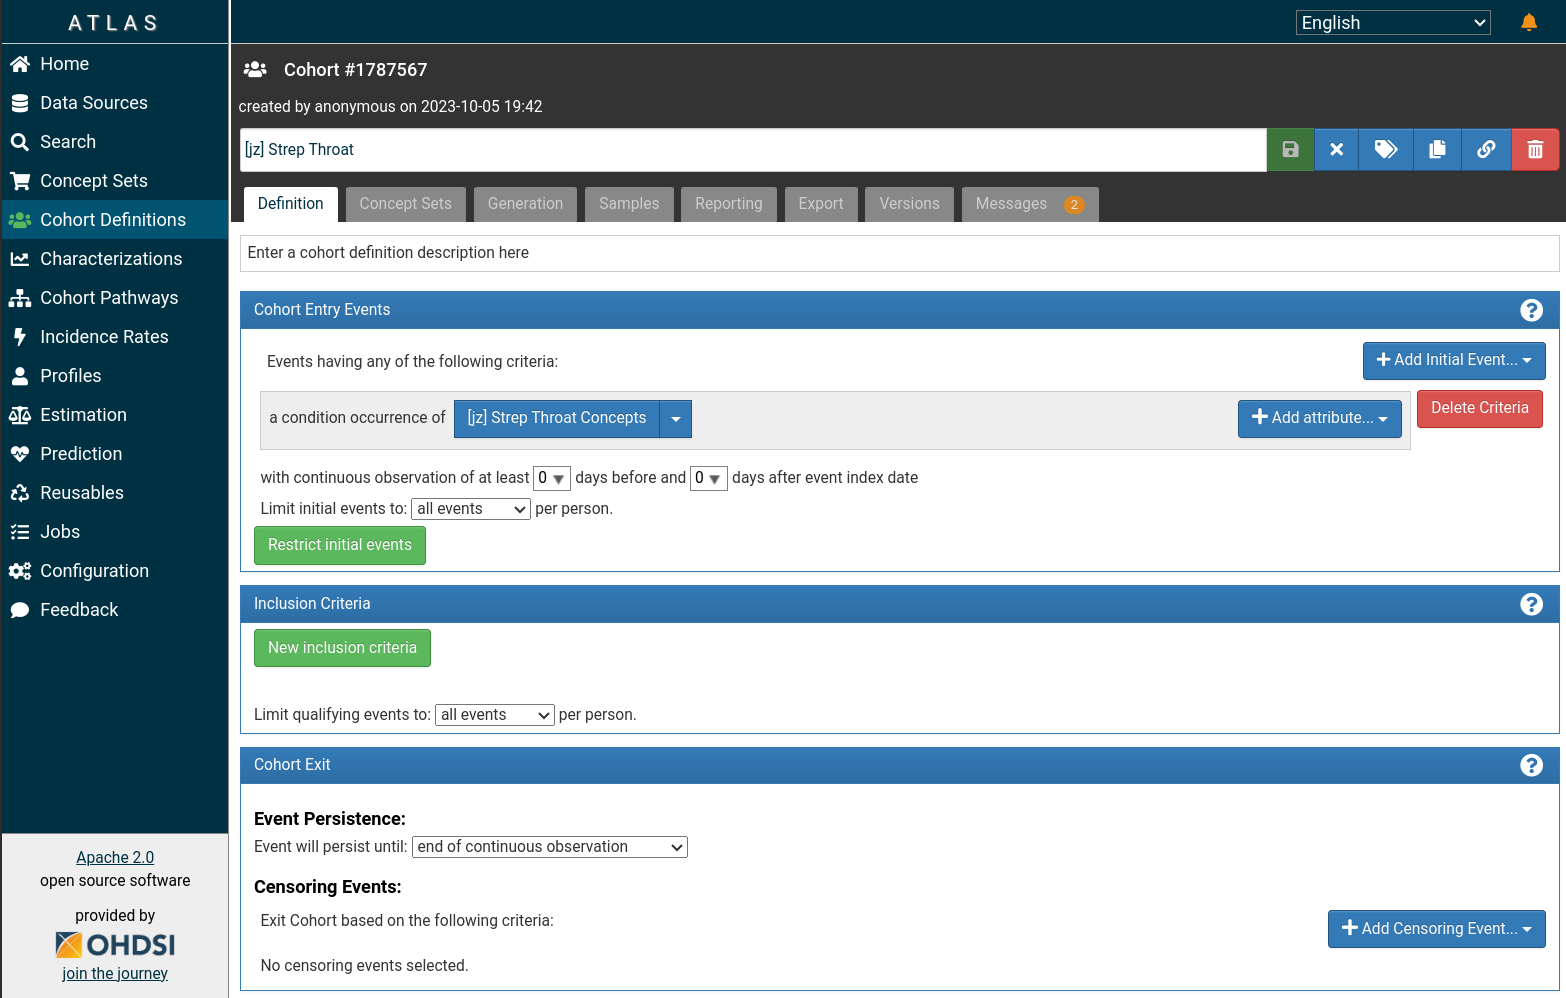
\includegraphics{./atlas_gui.png}

\subsection{Using a Cohort Definition To Build an Initial Cohort}

% EXPLAIN:: What is this doing here?
After having a strep throat phenotype definition defined using ATLAS, we can then execute the resulting computable phenotype definition against the \textit{Eunomia} database.

% TODO::HARD Maybe remove package imports and mention them within the caption instead
\begin{listing}[!ht]
\begin{minted}[breaklines,escapeinside=||,mathescape=true, numbersep=3pt, gobble=2, frame=lines, fontsize=\scriptsize, framesep=2mm]{julia}
model = oce.Model(cdm_version = v"5.3.1", 
              cdm_schema = "main",
              vocabulary_schema = "main", 
              results_schema = "main",
              target_schema = "main", 
              target_table = "cohort");

sql = oce.translate(cohort_expression, 
                dialect = :sqlite, 
                model = model, 
                cohort_definition_id = 1);
\end{minted}
\caption{\textbf{Creating a Cohort Using a Computable Phenotype Definition.} \textit{OHDSICohortExpressions.jl} (oce) ingests a computable phenotype definition to generate a cohort of patients. The JSON is translated into an intermediate SQL Syntax Tree, instantiated in SQL (SQLite) targeting an OMOP CDM v5.3.1 database, and then populates the database's cohort table.}
\label{listing:cohort_creation}
\end{listing}

\subsection{Characterizing Patient Populations}

% EXPLAIN:: What is this section doing?

\begin{listing}[!ht]
\begin{minted}[breaklines,escapeinside=||,mathescape=true, numbersep=3pt, gobble=2, frame=lines, fontsize=\scriptsize, framesep=2mm]{julia}
patients = occ.GetCohortSubjects(1, conn)

patients_race = occ.GetPatientRace(C.person_id, conn)
patients_gender = occ.GetPatientGender(C.person_id, conn)

patients_age_group = occ.GetPatientAgeGroup(
  C.person_id, 
  conn; 
)
\end{minted}
\caption{\textbf{Find Demographic Characteristics of Cohort.} Demographic properties of a cohort can be quickly queried from a database.}
\label{listing:demographics}
\end{listing}

\subsection{Calculating Crude Prevalence Rate}

% EXPLAIN::MEDIUM What is this section doing?

\begin{listing}[!ht]
\begin{minted}[breaklines,escapeinside=||,mathescape=true, numbersep=3pt, gobble=2, frame=lines, fontsize=\scriptsize, framesep=2mm]{julia}
strep_df = df.combine(patient_groups, df.nrow => :count)

# Creator code to process data and generate counts...

strep_df.prev = strep_df.count ./ strep_df.total_count 
\end{minted}
\caption{\textbf{Calculating crude prevalence rates.} Once demographic information is extracted, processing can be performed using tools such as \textit{DataFrames.jl} (df) to calculate metrics such as prevalence rates in a very straightforward manner.}
\label{listing:prevalence}
\end{listing}

Using this analytical approach, tabulation can be quickly conducted across patients.


% EXPLAIN::MEDIUM What is this section doing?

\begin{table}[!ht]
    \centering
    \begin{tabular}{|l|l|l|l|l|l|}
    \hline
        Race & Gender & Age Group & Cohort & Total & Prev. (\%) \\ \hline
        B/AA & F & 60 - 64 & 13 & 21 & 61.90 \\ \hline
        W & F & 50 - 54 & 59 & 111 & 53.15 \\ \hline
        W & F & 55 - 59 & 62 & 97 & 63.91 \\ \hline
        A & M & 80 - 84 & 6 & 10 & 60.00 \\ \hline
        UNK & F & 60 - 64 & 29 & 39 & 74.35 \\ \hline
        B/AA & M & 65 - 69 & 12 & 18 & 66.66 \\ \hline
    \end{tabular}
    \caption{\textbf{Example of a Strep Throat Prevalence Calculation.} This illustrates the sort of results one can quickly generate using the OHS. Note, that although the prevalence values in this table are based on synthetic data and are not realistic, the output looks very similar to what one could expect to generate.}
    \label{table:eunomia_prevalence}
\end{table}

\subsection{Summary of Results}

% TODO::HARD Create table for MIMIC III results
As seen in \ref{table:eunomia_prevalence}, informative results can be rapidly generated by this workflow relevant to observational health research.
Although the values shown in Table 2 are synthetic and the crude prevalence values themselves are meaningless, we can take a this approach and apply it directly to the MIMIC III dataset.
In Table 3, we can calculate across this dataset meaningful statistics that could later be further analyzed and drive further questioning (such as ...).

\section{Discussion}

\subsection{Advanced Features of the JuliaHealth Ecosystem}

% EXPLAIN::MEDIUM What is the overview of this section?
% EXPLAIN::MEDIUM What does each topic do?
\begin{enumerate}

\item Modularization of code and chaining

\item Distributed computing

\item Automatic generation of SQL from health packages

\end{enumerate}

% TODO::EASY Rename section
\subsubsection{Modularization of Code and Chaining}

% TODO::MEDIUM Make this more explicit about utilizing Julia's composition
An exciting emergent aspect of the JuliaHealth ecosystem that came about as a result of developing OMOPCDMCohortCreator.jl was the prospect of radical modularization and chaining of package functionalities together.
% TODO::MEDIUM Tie into currying more directly
% TODO::MEDIUM Check if I am mentioning currying correctly
We can leverage a unique property of Julia in that Julia supports partial evaluation of functions (also known as currying) to simplify repeated function calls to the same function over and over again.
% TODO::MEDIUM Rewrite this part in light of the previous sections 
For example, taking our workflow example from the earlier section where we characterized patients by race, gender, and age group, we can do a few "tricks" to modularize these characterization functions as follows:

% TODO::EASY Rework this section further
First, we'll take our original functions and fix a connection object to each of our cofactor functions.
This simplifies having to continuously pass forward a connection object and opens up the ability to chain together these functions simply:

% EXPLAIN::EASY Refactor this paragraph better or put most of it into the caption for the next code block
Second, as OMOPCDMCohortCreator.jl is built on top of DataFrames.jl and one has the option of creating a DataFrame with the result from every OCC function, we can use the package, Chain.jl.
This package abstracts away some of the explicit functionalities of DataFrames.jl but instead gives much easier ways to define a flow of functions:

\begin{listing}[!ht]
\begin{minted}[breaklines,escapeinside=||,mathescape=true, numbersep=3pt, gobble=2, frame=lines, fontsize=\scriptsize, framesep=2mm]{julia}
FGetPatientRace = Fix2(occ.GetPatientRace, conn)
FGetPatientGender = Fix2(occ.GetPatientGender, conn)
FGetPatientAgeGroup = Fix2(occ.GetPatientAgeGroup, conn)

CofactorPatients(patients) = @chain patients begin
    FGetPatientRace
    FGetPatientGender
    FGetPatientAgeGroup
end

CharacterizePatients(patients) = @chain patients begin
    _[:, df.Not(:person_id)]
    df.groupby(_, names(_))
    df.combine(_, df.nrow => :count)
    occ.ExecuteAudit
end

RunStudy(patients) = @chain patients begin
    CofactorPatients
    CharacterizePatients
end
\end{minted}
\caption{\textbf{Modularizing Study Code.} Using Julia's partial application abilities, connection objects can be fixed allowing study code to be readily modularized. Using the package, Chain.jl, occ and processing functions can be composed together to create modular study code.}
\label{listing:modular_study}
\end{listing}

In this way, future researchers using tools such as OMOPCDMCohortCreator.jl can create these more convenient abstractions.
% TODO::EASY Move this into the future discussion section
In fact, it could be a point of exploration in the future to build on top of OMOPCDMCohortCreator.jl even more abstracted and reusable functionalities to simplify ease of use while also enabling more readily auditable functionality.

% TODO::MEDIUM Move this into its own section
Finally, as these functions have now been fully modularized, these can now be readily distributed using Julia's distributed computing methods:

% TODO::HARD Redo example; I do not feel it is good
\begin{listing}[!ht]
\begin{minted}[breaklines,escapeinside=||,mathescape=true, numbersep=3pt, gobble=2, frame=lines, fontsize=\scriptsize, framesep=2mm]{julia}
import Distributed:
  @distributed 

result = @distributed (append!) for i in 1:10
   vals = 
      RunStudy(strep_patients[i*100 + 1:(i+1)*100, :])
   [vals]
end

vcat(result...) |> audit_patient_groups
\end{minted}
\caption{\textbf{Distributed Computation of a Study.} With occ, study code can be easily abstracted and modularized. Using Julia's native Distributed package, each module of a study can then be parallelized over patient cohorts.}
\label{listing:study_parallelization}
\end{listing}

Distributed computing here then allows a researcher to run multiple investigations at once as well as optimize performance to a given database.

\subsubsection{Auto-Generating SQL from JuliaHealth Commands}

% TODO::EASY Rephrase this sentence
One crucial aspect of the OHS is that it is unavoidable to work with databases that contain patient health information.
% TODO::EASY Rephrase this sentence better
% TODO::EASY Cite ANSI SQL
For better or worse, the tool that is used to best interact with these databases are SQL dialects that loosely follow consistently the ANSI SQL guidance.
% EXPLAIN::MEDIUM Highlight this more
% EXPLAIN::MEDIUM In what scenarios might using Julia may not be possible
To accomodate for this, several of the core tools developed in this sub-ecosystem generate SQL that can be used in the case where Julia may not be available in a given environment housing patient health data.
% EXPLAIN::MEDIUM Introduce this better
As an example, \textit{OMOPCDMCohortCreator.jl} functions build upon \textit{FunSQL.jl} allowing one to use a function such `GetPatientAgeGroup` without a connection object which would result in SQL.

\begin{listing}[!ht]
\begin{minted}[breaklines,escapeinside=||,mathescape=true, numbersep=3pt, gobble=2, frame=topline, fontsize=\scriptsize, framesep=2mm]{julia}
# Julia Input
occ.GetPatientAgeGroup([1]; age_groupings = [
                                              [0, 40], 
                                              [41, 80]
                                            ])

\end{minted}

\begin{minted}[breaklines,escapeinside=||,mathescape=true, numbersep=3pt, gobble=2, frame=bottomline, fontsize=\scriptsize, framesep=2mm]{sql}
# SQL Output
SELECT
  "PERSON_2"."person_id",
  (CASE 
    WHEN ("PERSON_2"."age" < 41) 
      THEN '0 - 40' 
    WHEN ("PERSON_2"."age" < 81) 
      THEN '41 - 80' END) AS "age_group"
FROM (
  SELECT
    "PERSON_1"."person_id",
    (2023 - "PERSON_1"."year_of_birth") AS "age"
  FROM "PERSON" AS "PERSON_1"
  WHERE ("PERSON_1"."person_id" IN (1))
) AS "PERSON_2"
\end{minted}
\caption{\textbf{Producing SQL from Julia Expression.} When occ functions are not passed a connection object, they can produce SQL representing the underyling query the Julia expression is executing.}
\label{listing:julia_sql}
\end{listing}

% TODO::MEDIUM Combine this section with the future directions section
\subsection{Strong Composition within JuliaHealth}

Within Julia, one aspect of the language that is often viewed as a technical problem within other languages emerges more as a social problem within Julia.
That problem is the problem of strong composition within Julia.
What composition within Julia is thought to be generally is that a user of Julia packages A and B can combine these packages oftentimes seamlessly together in such a way as to solve a problem that the original designers of A and B did not think about.
This has the virtue of Julia packages being strongly flexible to suit problems at hand but a discoverability problem where users developing these novel compositions may not share about these combinations.
As a result, there arise a paradox wherein strongly compositional systems, like Julia, simultaneously give rise to obfuscational logic.

Within JuliaHealth, this problem is an active area of exploration.
During the summer of 2023, this problem was one of the focuses of Google Summer of Code mentee, Fareeda Abdelazeez.
Originally, the project dealt with determining if another package in the JuliaHealth ecosystem was necessary to support prediction for patient outcomes.
Instead, what was realized instead is that what should be further investigated is novel compositions that can be viewed through the lens of JuliaHealth.
As shown in this workflow, although there were some packages that were made specifically for JuliaHealth, other packages that were not JuliaHealth specific were used alongside of it that composed flawlessly with the rest of the JuliaHealth OHS.

\subsection{Potential Future Directions}

% TODO::EASY Rephrase this introductory paragraph
JuliaHealth is now sufficiently at a stage of maturity where potential future researchers can leverage JuliaHealth's tools to conduct further future research or build upon existing architecture to target specific needs.
Some potential future directions that can be taken are as follows.

% TODO::MEDIUM This is where to introduce the paradox of composition
Due to the strong composition that exists within the JuliaHealth and broader Julia ecosystem, solutions may already exist for solving various health informatics related research.
However, what has consistently been a problem within the Julia ecosystem is the lack of sufficient documentation dedicated to describing these novel compositions and their application to various endeavors.
Future efforts can be dedicated to taking existing tools and reframing them in a JuliaHealth context to assist newcomers to Julia and JuliaHealth in determining how to explore and address problems that they are interested in.

% TODO::MEDIUM Combine this paragraph with the previous paragraph
% TODO::EASY Shorten this sentiment
Additionally, due to the composable and modular nature of the OHS, research analyses and visualizations can be decoupled and interchanged with one another.
Whereas in other ecosystems that make technologies for tools such as dashboards tightly coupled to analytics regimens, the subecosystem is mature enough to enable new users and developers to create analytics tools that can be separately woven into more graphical user interfaces.
For example, treatment pathways is a novel observational health approach to understand and visualize the care a patient receives within a care setting.
Only a few tools exist to visualize such hidden patient narratives but with the JuliaHealth ecosystem, the possibility of making tools that can interrogate patient care pathways more deeply could be fully realized.

% TODO::EASY Make this more about the flexible nature of the JuliaHealth organization
Furthermore, again exploiting the composition within the JuliaHealth ecosystem, as mentioned in the context of JuliaHealth and machine learning applications, future efforts could focus on developing fairness and bias auditing tools in patient datasets.
These tools could consider factors commonly explored in health equity literature like data completeness, demographic variables, and fairness algorithms. 

\section{Conclusion}

In conclusion, this paper has demonstrated the capabilities of the JuliaHealth OHS and its potential to further investigations in observational health research.
Although it is an ecosystem that is relatively new, its robustness allows for novel investigations to be pursued within this domain of research. 
% TODO::MEDIUM Mention how this allows JuliaHealth to solve more problems than what is present within JuliaHealth
Additionally, due to the strongly compositional nature of the Julia ecosystem, these JuliaHealth tools can readily compose with tooling to support in-depth statistical analyses, mathematical modeling, and visualization capacities.

% TODO::MEDIUM Rework this
In essence, the JuliaHealth ecosystem stands as a catalyst for transformative observational health research, poised to push the boundaries of innovation, collaboration, and standardization in the pursuit of better healthcare outcomes. As it continues to evolve, JuliaHealth emerges as a beacon of progress in the dynamic landscape of health informatics.

\section{Acknowledgements}

For this work, we would like to thank and recognize the following individuals and groups: 

\begin{enumerate}

  \item Dr. Jon Duke for his early support
  \item Kristin Kostka for being an early champion in trying novel ideas
  \item The JuliaHealth community and contributors for fearlessly trying to push boundaries on what observational health informatics can truly be
  \item Dilum Aluthge for helping this work find a home in JuliaHealth
  \item Adam Black for thinking through potential approaches
  \item Clark Evans and Kirill Simonov for being the pioneers of this work in Julia
  \item The Roux Institute's OHDSI Center for their encouragement

\end{enumerate}

% **************GENERATED FILE, DO NOT EDIT**************

\bibliographystyle{juliacon}
\bibliography{ref.bib}


\end{document}
